\documentclass[10pt]{article}

\usepackage{parskip}
\usepackage[margin=1in]{geometry} 
\usepackage{amsmath,amsthm,amssymb, graphicx, multicol, array}
\usepackage{makecell}
\usepackage{enumitem}
\usepackage{amssymb}
\usepackage{float}
\usepackage{href-ul}
 
\newcommand{\N}{\mathbb{N}}
\newcommand{\Z}{\mathbb{Z}}
 
\newenvironment{problem}[2][Problem]{\begin{trivlist}
\item[\hskip \labelsep {\bfseries #1}\hskip \labelsep {\bfseries #2.}]}{\end{trivlist}}

\begin{document}
 
\title{Use of binary variables}
\author{Jakob Sverre Alexandersen\\
GRA4154 Supply Chain Optimization with Mathematical Programming\\
Lecture 8}
\maketitle

\tableofcontents
\newpage

\section{TSP and Vehicle Routing Problem (VRP)}
\begin{itemize}
    \item Classic puzzles in mathematical programming 
    \item What is the most efficient way for 
    \begin{enumerate}
        \item a vehicle (TSP)
        \item a fleet of vehicles (VRP)
    \end{enumerate}
    to deliver goods to a specific set of customers?
    \item We have to leave a central depot, hitting various stops (customers), and return home
    \item The goal is to minimize the total cost -- usually measured by distance travelled, rime spent, or the number of trucks used -- while ensuring every customer gets served 
\end{itemize}
\subsection{TSP}
\begin{itemize}
    \item A company needs to plan the routes for a salesman visiting 11 customers, starting from the office and returning to the office 
    \item Each customer can be visited only once 
    \item Which route will minimize the total distance travelled?
\end{itemize}
\begin{figure}[H]
    \centering
    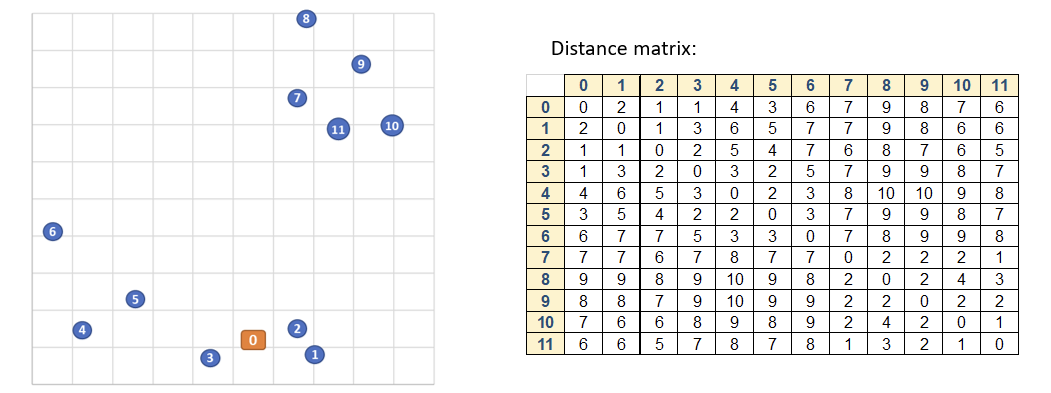
\includegraphics[width=0.8\textwidth]{2026-03-18-08-45-01.png}
\end{figure}
\newpage 
\textbf{Sets}
\begin{itemize}
    \item Let $\mathcal{G} = (\mathcal{V}, \mathcal{E}) $ be a complete graph where: 
    \item $\mathcal{V} = \{1, 2, \dots, n\} $: the set of $n $ customers
    \item $\mathcal{E} $: the set of all edges (pairs of customers)
\end{itemize}
\textbf{Parameters:}
\begin{itemize}
    \item $d_{i,j} $: distance from $i \text{ to } j $
\end{itemize}
\textbf{Variables:}
\begin{itemize}
    \item $x_{i,j} $: 1 if travelling from $i \text{ to } j $, 0 otherwise 
    \item $u_i $: the position of customer $i $ in the tour sequence (auxiliary continuous variable)
\end{itemize}
\textbf{Model}
\begin{gather}
    \min Z = \sum_{i\in \mathcal{V}}\sum_{j\in \mathcal{V}, j\neq i}d_{i,j}x_{i,j}\notag\\
    \text{s.t.}\notag\\
    \sum_{j\in \mathcal{V}, j\neq i} x_{i,j} = 1\quad\forall i\in \mathcal{V}\\
    \sum_{i\in \mathcal{V}, j\neq i} x_{i,j} = 1\quad\forall j\in \mathcal{V}\\
    u_i - u_j + nx_{i,j} \le n - 1\quad\forall i,j\in \{2, \dots, n\}, i\neq j\\
    1\le u_j \le n - 1\quad\forall i \in \{2, \dots, n\}
\end{gather}
\begin{enumerate}
    \item Leave every customer exactly once -- each node has exactly one outgoing edge 
    \item ``Enter'' every customer exactly once -- each node has exactly one incoming edge 
\end{enumerate}
These constraints ensure a set of tours that covers all customers, but they don't guarantee a single connected tour. Therefore we eliminate subtours with (3) and (4). This is the elegant trick -- if $x_{i, j} = 1 $ (i.e., we travel from $i $ to $ j $), then $u_j \ge u_i + 1$, enforcing a strict ordering of customers. A subtour would require a customer to appear ``before himself'' in the sequence -- a contradiction. Customer 1 is fixed as the depot, so $u_1 $ is excluded. 
\newpage 
\subsection{VRP}
In VRP, there is a given number of ``vehicles''. Each customer has a demand, and each vehicle may have limited capacity (in terms of total distance or in terms of cargo)

VRP can be modelled in different ways, and with different assumptions. Here is one example: 
\textbf{Sets and indices}
\begin{itemize}
    \item $\mathcal{V} = \{1, \dots, |\mathcal{V}|\} $: set of vehicles 
    \item $\mathcal{N} = \{0, 1, \dots, n\} $: set of nodes, where 0 is the depot and $\{1, \dots, n\} $ are customers 
\end{itemize}
\textbf{Parameters}
\begin{enumerate}
    \item $d_{i, j} $: distance from node $i \text{ to node } j $
    \item $q_j $: demand of customer $j $
    \item $Q $: capacity of each vehicle 
\end{enumerate}
\textbf{Decision variables} 
\begin{itemize}
    \item $x_{v, i, j} \in \{0, 1\} \quad\forall v\in \mathcal{V}, i\in \{0,\dots, n\}, j\in \{0,\dots, n\} $: 1 if vehicle $v $ travels from node $i $ to node $j $, else 0
\end{itemize}
\textbf{Model}
\begin{gather}
    \min Z = \sum_{v\in \mathcal{V}}\sum_{i = 0}^n\sum_{j = 0}^{n}d_{i, j}x_{i, j}\notag\\
    \text{s.t.}\notag\\
    \sum_{i = 0}^{n}\sum_{j = 1}^{n}q_jx_{v, i, j}\le Q\quad\forall v\in \mathcal{V}\\
    \sum_{j = 1}^{n}x_{v, 0, j} = 1\quad\forall v\in \mathcal{V}\\
    \sum_{i = 1}^{n}x_{v, i, 0} = 1\quad\forall v\in \mathcal{V}\\
    \sum_{j = 0}^{n}x_{v, i, j}\le 1\quad\forall v\in \mathcal{V}, i\in \{0, \dots, n\}\\
    \sum_{i = 0}^{n}x_{v, i, j}\le 1\quad\forall v\in \mathcal{V}, j\in \{0, \dots, n\}\\
    \sum_{v\in \mathcal{V}}\sum_{i = 0}^{n}x_{v, i, j} = 1\quad\forall j\in\{1,\dots, n\}\\
    \sum_{v\in \mathcal{V}}\sum_{j = 0}^{n}x_{v, i, j} = 1\quad\forall i\in\{1,\dots, n\}\\
    \sum_{j = 0}^{n}x_{v, i, j} = \sum_{j = 0}^{n}x_{v, j, i}\quad\forall v\in \mathcal{V}, i\in\{0, \dots, n\}\\
    x_{v, i, i} = 0 \quad\forall v\in \mathcal{V}, i\in \{0, \dots, n\}
\end{gather}
\newpage 

\begin{enumerate}[start=5]
    \item Capacity 
    \item One departure from depot 
    \item One arrival to depot 
    \item At most outgoing arc 
    \item At most incoming arc 
    \item Each customer visited once (arriving)
    \item Each customer visited once (departing)
    \item Flow conservation 
    \item No self-loops
\end{enumerate}
\textbf{Subtour elimination (by subtour length)}
\begin{align*}
    x_{v, i, j} + x_{v, j, i} &\le 1\quad\forall v\in \mathcal{V},\, i, j \in \{1, \dots, n\}\\
    x_{v, i, j} + x_{v, j, k} + x_{v, k, i} &\le 1\quad\forall v\in \mathcal{V},\, i, j, k \in \{1, \dots, n\}\\
    x_{v, i, j} + x_{v, j, k} + x_{v, k, l} + x_{v, l, i} &\le 1\quad\forall v\in \mathcal{V},\, i, j, k, l \in \{1, \dots, n\}\\
    x_{v, i, j} + x_{v, j, k} + x_{v, k, l} + x_{v, l, m} + x_{v, m, i} &\le 1\quad\forall v\in \mathcal{V},\, i, j, k, l, m \in \{1, \dots, n\}
\end{align*} 
\subsubsection{The ``savings'' heuristic, as suggested by Clarke and Wright}

Assume the following cost matrix:
\begin{figure}[H]
    \centering
    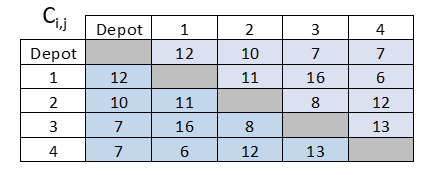
\includegraphics[width=0.4\textwidth]{2026-03-18-09-11-38.png}
\end{figure}
and the following customer demands 
\begin{center}
    \begin{tabular}{|c|c|}
        \hline 
        \textbf{Customer} & \textbf{Demand}\\\hline 
        1 & 10 \\\hline 
        2 & 8 \\\hline 
        3 & 5 \\\hline 
        4 & 16 \\\hline 
    \end{tabular}
\end{center}
Assume that the capacity of the truck is 32 pallets. First, combine according to the ranking list: 1 and 4: total cargo is 26 pallets. 

Next on the list is combining 1 and 2, i.e., add customer 2 to the existing route if feasible. But \underline{not} feasible since the remaining capacity of the truck (6 pallets) is lower than the demand (8 pallets) of customer 2. 

Next on the list is a combination of 2 and 3. This will be a separate route since 2 and 3 are not on the first route. A route consisting of 2 and 3 is feasible since the total demand (13 pallets) does not exceed the truck's capacity. 

All customers are now assigned to a route. Hence, the heuristic is finished. 

The first route will then consist of (1) and (4). The total cost is $12 + 6 + 7 = 25 $ (depot to 1 to 4 to depot). The second route will consist of (2) and (3). Total cost: $10 + 8 + 7 = 25 $ (depot to 2 to 3 to depot). The total cost for this solution is $25 + 25 = 50 $
\newpage 
\textbf{Sets and Indices}
\begin{itemize}
    \item $\mathcal{N} = \{1,\dots, n\} $: customers 
    \item $\mathcal{N}_0 = \{0\}\cup \mathcal{N} $: all nodes, depot indexes by 0
    \item $\mathcal{S} = \{(i, j) | i, j \in \mathcal{N}, i < j\} $: set of candidate savings pairs 
\end{itemize}
\textbf{Parameters}
\begin{itemize}
    \item $d_{i, j} $: distance between nodes $i \text{ and } j $
    \item $q_i $: demand of customer $i\in \mathcal{N} $
    \item $Q $: vehicle capacity
    \item $s_{i, j} = d_{0, i} + d_{0, j} - d_{i, j} $: saving from merging $i \text{ and } j $ into one route 
\end{itemize}
\textbf{Decision Variable}
\begin{itemize}
    \item $y_{i, j}\in \{0, 1\}\quad\forall (i, j)\in \mathcal{S} $: 1 if the saving $(i, j) $ is realized, i.e., customers $i \text{ and } j $ are placed on the same route with the depot-return between them eliminated 
\end{itemize}
\textbf{Objective function}
\begin{gather}
    \max Z = \sum_{(i, j)\in \mathcal{S}}s_{i, j}y_{i, j}\notag\\
    \text{s.t.}\notag \\
    \sum_{j\in \mathcal{N}\setminus \{i\}}y_{i, j}\le 2\quad\forall i\in \mathcal{N}\\
    \sum_{j\in \mathcal{N}\setminus \{i\}}y_{i, j}\le 1\quad\forall i\in \mathcal{N}\\
    \sum_{i\in mc}
\end{gather}
\end{document}